% ============================================================
%  DISCOVERY CURRICULUM — Journey 1, Module 2
%  "Functions as Relationships"
%  Compile with: pdflatex J1_M2.tex  (run twice for references)
% ============================================================

\documentclass[12pt, a4paper]{article}

\usepackage[a4paper, top=2.8cm, bottom=2.8cm, left=3.0cm, right=2.5cm, includeheadfoot, headheight=15pt]{geometry}
\usepackage{amsmath, amsthm}
\usepackage[charter, cal=cmcal]{mathdesign}
\usepackage[scaled=0.92]{helvet}
\usepackage{xcolor}
\usepackage{tcolorbox}
\tcbuselibrary{skins, breakable, theorems}
\usepackage{enumitem}
\usepackage{graphicx}
\usepackage{tikz}
\usetikzlibrary{arrows.meta, positioning, calc}
\usepackage{pgfplots}
\pgfplotsset{compat=1.18}
\usepackage{booktabs}
\usepackage{array}
\usepackage{fancyhdr}
\usepackage{titlesec}
\usepackage{parskip}
\usepackage{microtype}
\usepackage{hyperref}
\hypersetup{colorlinks=true, linkcolor=NavyBlue, urlcolor=NavyBlue}

% ── Colours ─────────────────────────────────────────────────
\definecolor{NavyBlue}{HTML}{1E3A8A}
\definecolor{MidBlue}{HTML}{2E6DA4}
\definecolor{Gold}{HTML}{D97706}
\definecolor{LightBlue}{HTML}{EFF6FF}
\definecolor{LightGold}{HTML}{FEF3C7}
\definecolor{DarkGrey}{HTML}{334155}
\definecolor{BoxGreen}{HTML}{F0FDF4}
\definecolor{SoftRed}{HTML}{FFF1F2}
\definecolor{SidebarGrey}{HTML}{F8FAFC}

% ── Section formatting ───────────────────────────────────────
\titleformat{\section}{\Large\bfseries\color{NavyBlue}}{}{0em}{}[{\color{MidBlue}\vspace{2pt}\rule{\linewidth}{1.5pt}}]
\titleformat{\subsection}{\large\bfseries\color{MidBlue}}{}{0em}{}
\titleformat{\subsubsection}{\normalsize\bfseries\color{Gold}}{}{0em}{}

% ── Header / Footer ─────────────────────────────────────────
\pagestyle{fancy}
\fancyhf{}
\fancyhead[L]{\small\color{DarkGrey}\textit{Discovery Curriculum}}
\fancyhead[R]{\small\color{DarkGrey}\textit{Journey 1 $\cdot$ Module 2}}
\fancyfoot[C]{\small\color{MidBlue}\thepage}
\renewcommand{\headrulewidth}{0.4pt}

% ── Environments (tcolorbox Unification) ─────────────────────

% Puzzle box — opening problem
\newtcolorbox{puzzlebox}[1][]{
  enhanced, breakable,
  colback=NavyBlue!5, colframe=NavyBlue,
  boxrule=0pt, leftrule=2.5pt,
  sharp corners,
  left=12pt, right=10pt, top=10pt, bottom=10pt,
  before skip=14pt, after skip=10pt,
  #1
}

% Discovery box — moment of crystallisation
\newtcolorbox{discoverybox}[1][]{
  enhanced, breakable,
  colback=LightGold, colframe=Gold,
  boxrule=0pt, leftrule=2.5pt,
  sharp corners,
  left=12pt, right=10pt, top=10pt, bottom=10pt,
  before skip=14pt, after skip=10pt,
  #1
}

% Name box — formal definition reveal
\newtcolorbox{namebox}[1][]{
  enhanced, breakable,
  colback=LightBlue, colframe=MidBlue,
  boxrule=0.8pt,
  arc=4pt,
  left=12pt, right=10pt, top=10pt, bottom=10pt,
  before skip=14pt, after skip=10pt,
  #1
}

% Reflection box
\newtcolorbox{reflectionbox}[1][]{
  enhanced, breakable,
  colback=BoxGreen, colframe=DarkGrey!35,
  boxrule=0.8pt,
  arc=4pt,
  left=12pt, right=10pt, top=10pt, bottom=10pt,
  before skip=14pt, after skip=10pt,
  #1
}

% Thought provocation — inline philosophical aside
\newtcolorbox{thought}[1][]{
  enhanced, breakable,
  colback=SidebarGrey, colframe=Gold,
  boxrule=0pt, leftrule=1.5pt,
  sharp corners,
  left=10pt, right=10pt, top=7pt, bottom=7pt,
  before skip=10pt, after skip=10pt,
  #1
}

% Problem counter
\newcounter{problem}
\newenvironment{problem}[1][]{%
  \refstepcounter{problem}%
  \par\vspace{6pt}%
  \noindent\textbf{\color{MidBlue}Problem \theproblem}%
  \ifx&#1&\else\ \textit{(#1)}\fi\textbf{.}\enskip
}{\par\vspace{4pt}}

% Deep problem counter
\newcounter{deepproblem}
\newenvironment{deepproblem}[1][]{%
  \refstepcounter{deepproblem}%
  \par\vspace{6pt}%
  \noindent\textbf{\color{NavyBlue}$\bigstar$\ Deep Problem \thedeepproblem}%
  \ifx&#1&\else\ \textit{(#1)}\fi\textbf{.}\enskip
}{\par\vspace{4pt}}

% Exercise counter
\newcounter{exercise}
\newenvironment{exercise}[1][]{%
  \refstepcounter{exercise}%
  \par\vspace{6pt}%
  \noindent\textbf{\color{Gold}Exercise \theexercise}%
  \ifx&#1&\else\ \textit{(#1)}\fi\textbf{.}\enskip
}{\par\vspace{4pt}}


% ============================================================
\begin{document}
% ============================================================

% ── Cover ───────────────────────────────────────────────────
\thispagestyle{empty}
\begin{center}
{\small\color{MidBlue}\textbf{DISCOVERY CURRICULUM}\quad$\cdot$\quad\textbf{JOURNEY 1: REPRESENTATION}}

\vspace{0.6cm}
{\color{NavyBlue}\rule{\linewidth}{2pt}}
\vspace{0.5cm}

{\Huge\bfseries\color{NavyBlue}Module 2}\\[0.3cm]
{\LARGE\bfseries\color{MidBlue}Functions as Relationships}\\[0.4cm]
{\color{Gold}\rule{0.4\linewidth}{1.2pt}}\\[0.4cm]
{\large\itshape\color{DarkGrey}Two things can be related without one controlling the other.\\[0.15cm]
When does a relationship become something you can depend on?}

\vspace{1cm}
\begin{tabular}{rl}
\color{DarkGrey}\textbf{Journey}           & Journey 1 --- Representation \\[4pt]
\color{DarkGrey}\textbf{Module}            & 2 of 6 \\[4pt]
\color{DarkGrey}\textbf{Prerequisites}     & Module 1 (functions, domain, composition) \\[4pt]
\color{DarkGrey}\textbf{You will discover} & Inverse functions, bijections, function spaces \\[4pt]
\color{DarkGrey}\textbf{Format}            & 8 problems $+$ 3 deep problems $\approx$ 12--14 pages \\
\end{tabular}

\vspace{1cm}
{\color{NavyBlue}\rule{\linewidth}{2pt}}
\end{center}

\vspace{0.6cm}

\noindent\textbf{Recap of Module 1.}
In Module~1 you discovered that a \textbf{function} is a rule assigning to each element of a domain exactly one output. You saw that this ``exactly one'' condition is not a formality --- it is what makes a rule reliable enough to reason with. You also encountered \textbf{composition}: chaining two functions so the output of one feeds into the input of the next.

\medskip
This module asks a deeper question: \textit{can you go backwards?} Given the output of a function, can you always recover the input? And what does the answer tell us about the nature of information, reversibility, and the structure of relationships?

\newpage

% ============================================================
\section{Part 1 \texorpdfstring{---}{--} The Puzzle}
% ============================================================

\begin{puzzlebox}
\textbf{The Opening Puzzle.}

A government official is encoding secret messages. Their encoding rule is simple: take a number, multiply by 3, then add 7.

\medskip
They send you the encoded number \textbf{28}.

\medskip
\textbf{Question.} What was the original number? Can you always recover it, no matter what encoded number you receive? Now suppose the encoding rule had been: ``take a number and square it.'' You receive \textbf{25}. What was the original number now? Is there always a unique answer?
\end{puzzlebox}

\medskip
The two encoding rules behave very differently. One can be perfectly undone. The other cannot always be --- at least not without extra information. This difference is not accidental. It runs deep into the structure of what a function is, and it connects to questions that matter far beyond mathematics: encryption, data compression, invertible physical processes, and even the thermodynamic arrow of time.

\begin{thought}
\textbf{Reversibility in physics.}
The laws of classical mechanics are time-reversible: if you film a billiard ball collision and play it backwards, the reversed film obeys the same laws. But in practice, you cannot unscramble an egg. Something is lost. The mathematical language for this distinction --- between processes that can and cannot be undone --- is exactly the language we are about to develop. A function that can be reversed is a very special kind of function. It preserves information perfectly. Most functions do not.
\end{thought}

% ============================================================
\section{Part 2 \texorpdfstring{---}{--} Exploration}
% ============================================================

\subsection{Step 1: Going backwards}

\begin{problem}
\label{prob:inverse_linear}
Consider the function $f(x) = 3x + 7$.
\begin{enumerate}[label=(\alph*), topsep=2pt]
  \item Compute $f(3)$, $f(0)$, $f(-2)$.
  \item You are told $f(x) = 28$. Find $x$. Describe your process.
  \item You are told $f(x) = y$ for some unknown $y$. Express $x$ in terms of $y$.
  \item The expression you found in (c) is itself a function of $y$. Call it $g(y)$. Compute $g(f(3))$. What do you get?
  \item Compute $f(g(10))$. What do you get? Is this a coincidence?
\end{enumerate}
\end{problem}

\begin{problem}
\label{prob:inverse_square}
Now consider the function $h(x) = x^2$.
\begin{enumerate}[label=(\alph*), topsep=2pt]
  \item Compute $h(3)$ and $h(-3)$. What do you notice?
  \item You are told $h(x) = 25$. Find all possible values of $x$.
  \item You are told $h(x) = -4$. Find all possible values of $x$.
  \item Why can you not define a single reliable ``reverse function'' for $h$ on all of $\mathbb{R}$?
  \item If you restrict the domain of $h$ to $[0, \infty)$, does the problem disappear? Explain carefully.
\end{enumerate}
\end{problem}

\medskip
Problems~\ref{prob:inverse_linear} and~\ref{prob:inverse_square} reveal a fundamental asymmetry. Some functions are reversible everywhere. Others are not. The difference lies in a structural property of the function itself.

\begin{thought}
\textbf{What information does a function destroy?}
When you apply $h(x) = x^2$ to the numbers $3$ and $-3$, both give 9. The function has \emph{collapsed} two distinct inputs into a single output. The information about which input you started with is gone --- you cannot recover it from the output alone. Functions that collapse inputs in this way are \emph{not} reversible. Functions that keep every input distinct in the output --- that never collapse two things into one --- are the reversible ones. This idea, that functions can destroy or preserve information, is one of the central organising ideas of modern mathematics and information theory.
\end{thought}

\subsection{Step 2: Diagrams of functions}

It helps to think of functions not just as formulas, but as \emph{arrows between sets}.

\begin{center}
\begin{tikzpicture}[
  every node/.style={font=\small},
  set/.style={ellipse, draw=MidBlue, thick, minimum width=2.2cm, minimum height=3cm},
  arr/.style={-{Stealth[length=5pt]}, MidBlue, thick}
]
% Domain
\node[set, label=above:{\color{NavyBlue}$A$ (domain)}] (A) at (0,0) {};
\foreach \y/\val in {0.8/a_1, 0/a_2, -0.8/a_3} {
  \node[circle, fill=MidBlue, inner sep=2pt] (d\val) at (-0.1,\y) {};
  \node[left=2pt of d\val] {$\val$};
}
% Codomain
\node[set, label=above:{\color{NavyBlue}$B$ (codomain)}] (B) at (5.5,0) {};
\foreach \y/\val in {0.8/b_1, 0/b_2, -0.8/b_3} {
  \node[circle, fill=Gold, inner sep=2pt] (c\val) at (5.6,\y) {};
  \node[right=2pt of c\val] {$\val$};
}
% Arrows
\draw[arr] (da_1) -- (cb_1);
\draw[arr] (da_2) -- (cb_3);
\draw[arr] (da_3) -- (cb_2);
% Label
\node at (2.75, 1.8) {\color{DarkGrey}\textit{function $f$}};
\draw[-{Stealth[length=6pt]}, DarkGrey, thick] (1.2, 1.6) -- (4.3, 1.6);
\end{tikzpicture}
\end{center}

\begin{problem}
\label{prob:arrow_diagrams}
Each diagram below shows a rule assigning outputs (right set) to inputs (left set). For each one:
\begin{itemize}[topsep=2pt]
  \item Is it a valid function? (Does every input have exactly one output?)
  \item If it is a function, can you define a reverse rule from the right set back to the left? Is the reverse rule also a valid function?
\end{itemize}

\begin{center}
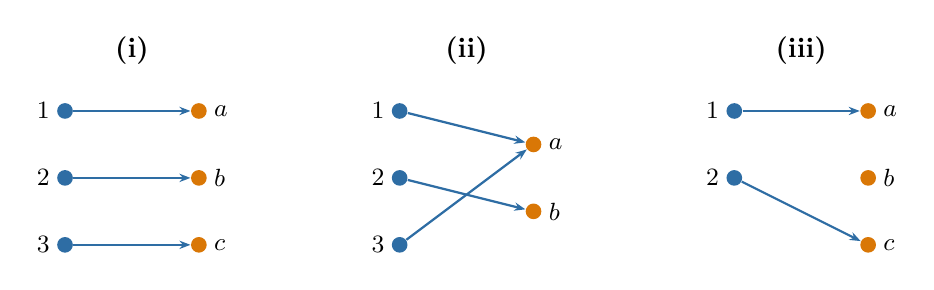
\begin{tikzpicture}[scale=0.85,
  dot/.style={circle, fill, inner sep=2pt},
  arr/.style={-{Stealth[length=4pt]}, MidBlue, thick}
]
% --- Diagram (i) ---
\node at (1.5, 3.4) {\textbf{(i)}};
\foreach \y/\l in {2.5/1, 1.5/2, 0.5/3} {
  \node[dot, MidBlue] (Li\l) at (0.5, \y) {};
  \node[left=2pt, font=\small] at (0.5,\y) {$\l$};
}
\foreach \y/\l in {2.5/a, 1.5/b, 0.5/c} {
  \node[dot, Gold] (Ri\l) at (2.5, \y) {};
  \node[right=2pt, font=\small] at (2.5,\y) {$\l$};
}
\draw[arr] (Li1) -- (Ria);
\draw[arr] (Li2) -- (Rib);
\draw[arr] (Li3) -- (Ric);

% --- Diagram (ii) ---
\node at (6.5, 3.4) {\textbf{(ii)}};
\foreach \y/\l in {2.5/1, 1.5/2, 0.5/3} {
  \node[dot, MidBlue] (Lii\l) at (5.5, \y) {};
  \node[left=2pt, font=\small] at (5.5,\y) {$\l$};
}
\foreach \y/\l in {2.0/a, 1.0/b} {
  \node[dot, Gold] (Rii\l) at (7.5, \y) {};
  \node[right=2pt, font=\small] at (7.5,\y) {$\l$};
}
\draw[arr] (Lii1) -- (Riia);
\draw[arr] (Lii2) -- (Riib);
\draw[arr] (Lii3) -- (Riia);

% --- Diagram (iii) ---
\node at (11.5, 3.4) {\textbf{(iii)}};
\foreach \y/\l in {2.5/1, 1.5/2} {
  \node[dot, MidBlue] (Liii\l) at (10.5, \y) {};
  \node[left=2pt, font=\small] at (10.5,\y) {$\l$};
}
\foreach \y/\l in {2.5/a, 1.5/b, 0.5/c} {
  \node[dot, Gold] (Riii\l) at (12.5, \y) {};
  \node[right=2pt, font=\small] at (12.5,\y) {$\l$};
}
\draw[arr] (Liii1) -- (Riiia);
\draw[arr] (Liii2) -- (Riiic);
\end{tikzpicture}
\end{center}
\end{problem}

\begin{problem}
\label{prob:reverse_existence}
For each function below, determine whether a reverse function exists on the given domain and codomain. If it does, write it explicitly. If it does not, explain precisely why not.
\begin{enumerate}[label=(\alph*), topsep=2pt]
  \item $f : \mathbb{R} \to \mathbb{R}$, \quad $f(x) = 2x - 5$
  \item $g : \mathbb{R} \to \mathbb{R}$, \quad $g(x) = x^3$
  \item $h : [0, \infty) \to [0, \infty)$, \quad $h(x) = x^2$
  \item $k : \mathbb{R} \to (0, \infty)$, \quad $k(x) = e^x$
  \item $m : \{1, 2, 3\} \to \{1, 4, 9\}$, \quad $m(x) = x^2$
\end{enumerate}
\end{problem}

\subsection{Step 3: The graph as a picture of a function}

Functions can be drawn. The graph of $f$ is the set of all points $(x, f(x))$ in the plane. This gives us a visual way to check properties of functions.

\begin{problem}
\label{prob:vline}
Consider the following statement: \textit{A curve in the plane is the graph of a function from $\mathbb{R}$ to $\mathbb{R}$ if and only if every vertical line crosses the curve at most once.}

\begin{enumerate}[label=(\alph*), topsep=2pt]
  \item Explain why this statement is true. What does a vertical line represent? What does it mean for it to cross the curve more than once?
  \item A circle centred at the origin with radius 1 is given by $x^2 + y^2 = 1$. Is this a function $y = f(x)$? Apply the vertical line test. What goes wrong?
  \item Can you express the top half of the circle as a function? The bottom half?
  \item Now consider: \textit{a curve is the graph of an invertible function if and only if every vertical line and every horizontal line crosses the curve at most once.} Explain this statement. What does the horizontal line test detect?
\end{enumerate}
\end{problem}

\begin{center}
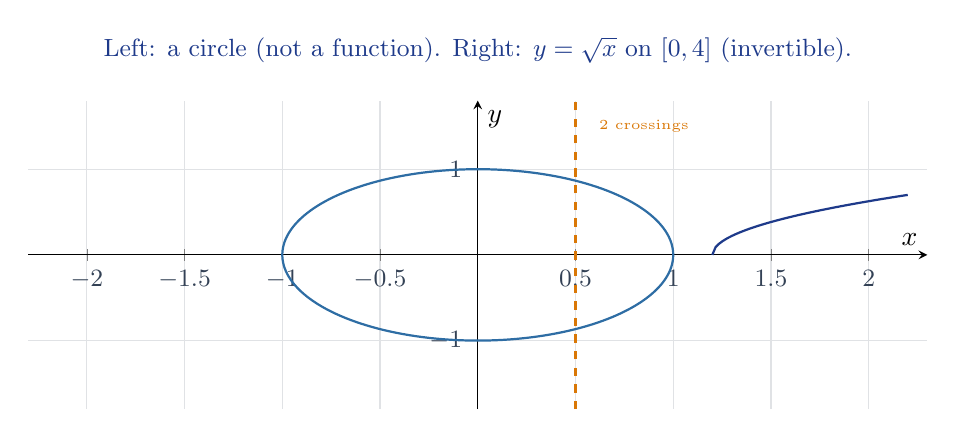
\begin{tikzpicture}
\begin{axis}[
  width=13cm, height=5.5cm,
  axis lines=center,
  xlabel={$x$}, ylabel={$y$},
  xmin=-2.3, xmax=2.3, ymin=-1.8, ymax=1.8,
  tick label style={font=\small, color=DarkGrey},
  grid=major, grid style={DarkGrey!15},
  title={\small\color{NavyBlue}Left: a circle (not a function). Right: $y = \sqrt{x}$ on $[0,4]$ (invertible).},
  title style={yshift=4pt},
]
% Circle
\addplot[MidBlue, thick, domain=0:360, samples=180] ({cos(x)}, {sin(x)});
\addplot[Gold, dashed, thick] coordinates {(0.5,-1.8)(0.5,1.8)};
\node[color=Gold, font=\tiny] at (axis cs:0.85,1.5) {2 crossings};
% sqrt on right
\addplot[NavyBlue, thick, domain=1.2:2.2, samples=60] {0.7*sqrt(x-1.2)};
\end{axis}
\end{tikzpicture}
\end{center}

\subsection{Step 4: Functions as inputs and outputs}

So far, functions have taken numbers as inputs and returned numbers as outputs. But there is no reason to stop there.

\begin{problem}
\label{prob:higher_order}
Consider the following rules. For each one, determine what kind of object is the input and what kind is the output.
\begin{enumerate}[label=(\alph*), topsep=2pt]
  \item ``Given a function $f : \mathbb{R} \to \mathbb{R}$ that is differentiable, produce its derivative $f'$.''
  \item ``Given a function $f : [0,1] \to \mathbb{R}$ that is integrable, produce the number $\displaystyle\int_0^1 f(x)\,dx$.''
  \item ``Given two functions $f$ and $g$, produce their composition $g \circ f$.''
  \item ``Given a function $f : \mathbb{R} \to \mathbb{R}$, produce the function $F(x) = f(x) + f(-x)$.''
  \item In cases (a) and (b): what is the ``domain'' of the rule? That is, which functions can be given as inputs?
\end{enumerate}
\end{problem}

\begin{thought}
\textbf{Functions all the way down.}
When you take the derivative of a function, you are applying a function to a function. The derivative is not just a formula --- it is a \emph{rule that takes functions as input and produces functions as output}. Mathematicians call this a \textbf{functional} or an \textbf{operator}. The Laplace transform, which you will meet in Journey~6, is a function whose inputs and outputs are both functions. So is the Fourier transform. So is the operator that takes a quantum state and produces the expected energy. The language you are building right now --- functions, domains, compositions --- is the language in which all of these ideas are expressed.

Once you realise that functions can themselves be objects that are inputs and outputs, you have crossed an important threshold. You are no longer thinking only about numbers. You are thinking about \emph{structures}.
\end{thought}

\begin{problem}
\label{prob:function_space}
Let $\mathcal{F}$ denote the set of all functions from $\mathbb{R}$ to $\mathbb{R}$.
\begin{enumerate}[label=(\alph*), topsep=2pt]
  \item If $f, g \in \mathcal{F}$, define $(f + g)(x) = f(x) + g(x)$. Is $f + g$ also in $\mathcal{F}$?
  \item Define $(cf)(x) = c \cdot f(x)$ for a constant $c \in \mathbb{R}$. Is $cf$ also in $\mathcal{F}$?
  \item What is the ``zero element'' of $\mathcal{F}$ --- a function $z$ such that $f + z = f$ for all $f$?
  \item Does $\mathcal{F}$ remind you of any other mathematical structure you have encountered? (Think about how vectors behave.) Write down as many similarities as you can find.
\end{enumerate}
\end{problem}

\medskip
Problem~\ref{prob:function_space} is a hint at something large. The set of all functions, under addition and scalar multiplication, behaves remarkably like the vectors you studied in geometry. This is not a coincidence. In Journey~3 you will discover that functions \emph{are} vectors --- in an infinite-dimensional space. The Fourier transform is, at its core, a change of basis in that space.

% ============================================================
\section{Part 3 \texorpdfstring{---}{--} Discovery}
% ============================================================

\begin{discoverybox}
\textbf{What have we built?}

This module has uncovered three things.

\medskip
\textbf{First.} Some functions can be perfectly reversed; others cannot. The reversible ones are exactly those that never map two different inputs to the same output (injective) \emph{and} that fill up the entire codomain (surjective). Together: bijective.

\medskip
\textbf{Second.} The graph of a function gives a visual language for these properties: the vertical line test checks that it is a function; the horizontal line test checks that it is invertible.

\medskip
\textbf{Third.} Functions can themselves be the inputs and outputs of other functions. The collection of all functions is a rich mathematical object in its own right.

\medskip
\textbf{Before reading on:} Try to write a precise definition of the \emph{inverse function} of a bijection $f : A \to B$. What properties must it have? How would you verify that a proposed reverse function is correct?
\end{discoverybox}

% ============================================================
\section{Part 4 \texorpdfstring{---}{--} Naming the Ideas}
% ============================================================

\begin{namebox}
\textbf{Inverse functions.}

Let $f : A \to B$ be a bijection. The \textbf{inverse function} $f^{-1} : B \to A$ is the unique function satisfying
\[
  f^{-1}(f(a)) = a \quad \text{for all } a \in A,
  \qquad\text{and}\qquad
  f(f^{-1}(b)) = b \quad \text{for all } b \in B.
\]
In other words: $f^{-1} \circ f = \mathrm{id}_A$ and $f \circ f^{-1} = \mathrm{id}_B$, where $\mathrm{id}$ denotes the identity function $\mathrm{id}(x) = x$.

Inverses exist \emph{if and only if} $f$ is bijective. If $f$ fails to be injective (two inputs share an output), there is no way to reverse it unambiguously. If $f$ fails to be surjective (some outputs are never reached), the reverse has no value to assign at those points.

\medskip
\textbf{Warning.} The notation $f^{-1}$ is overloaded. For a real-valued function $f$, the notation $f^{-1}(x)$ means the inverse function, not $\tfrac{1}{f(x)}$. Context always determines which is meant.
\end{namebox}

\begin{namebox}
\textbf{Higher-order functions and operators.}

A \textbf{higher-order function} (or \textbf{operator}) is a function whose inputs, outputs, or both are themselves functions. Examples:
\begin{itemize}[topsep=4pt]
  \item The differentiation operator $\mathcal{D} : f \mapsto f'$, taking differentiable functions to functions.
  \item The integration functional $I : f \mapsto \displaystyle\int_0^1 f(x)\,dx$, taking integrable functions to real numbers.
  \item The shift operator $T_h : f \mapsto g$ where $g(x) = f(x - h)$, translating a function horizontally.
\end{itemize}

\medskip
\textbf{Function spaces.} The collection $\mathcal{F}$ of all functions $f : \mathbb{R} \to \mathbb{R}$ equipped with pointwise addition and scalar multiplication is a \textbf{vector space}. This is not a metaphor --- it satisfies exactly the same axioms as geometric vectors. Subsets of $\mathcal{F}$ with special properties (continuous functions, differentiable functions, square-integrable functions) are \textbf{subspaces}. This will be developed fully in Journey~3.
\end{namebox}

\medskip
\noindent\textbf{A remark on notation.}
The notation $f : A \to B$ was made standard largely through the influence of \textbf{Nicolas Bourbaki} --- a pseudonymous collective of French mathematicians active from the 1930s onwards, who undertook to rewrite all of mathematics with rigorous, unified notation. Before Bourbaki, notation for functions varied wildly across authors and countries. The clarity of modern mathematical writing owes a great deal to this effort.

\begin{thought}
\textbf{On the meaning of $f^{-1}$.}
When a function has an inverse, something philosophically significant is happening: the function preserves all the information in its input. Nothing is lost. Applying $f$ and then $f^{-1}$ brings you back to exactly where you started. In physics, processes with this property are called \emph{reversible}. In information theory, they are \emph{lossless}. The mathematical condition --- bijectivity --- is the precise formulation of a very general idea: that some transformations preserve structure completely, and others do not. Most of the interesting mathematics in this curriculum is about understanding this distinction in increasingly subtle settings.
\end{thought}

% ============================================================
\section{Part 5 \texorpdfstring{---}{--} Deep Problems}
% ============================================================

\begin{deepproblem}
Let $f : A \to B$ and $g : B \to C$ be functions.
\begin{enumerate}[label=(\alph*)]
  \item Suppose both $f$ and $g$ are bijections. Prove that $g \circ f : A \to C$ is also a bijection, and find a formula for $(g \circ f)^{-1}$ in terms of $f^{-1}$ and $g^{-1}$.
  \item Suppose $g \circ f$ is injective. Must $f$ be injective? Must $g$ be injective? Prove or give a counterexample for each.
  \item Suppose $g \circ f$ is surjective. Must $g$ be surjective? Must $f$ be surjective? Prove or give a counterexample for each.
  \item Summarise your findings in (b) and (c) as a single clean theorem about the composition of functions.
\end{enumerate}
\end{deepproblem}

\begin{deepproblem}[Fixed points]
A \textbf{fixed point} of a function $f : A \to A$ is an element $a \in A$ such that $f(a) = a$.
\begin{enumerate}[label=(\alph*)]
  \item Find all fixed points of $f(x) = x^2 - x + 1$ on $\mathbb{R}$.
  \item Find all fixed points of $f(x) = \cos(x)$ on $\mathbb{R}$. (You may estimate numerically.)
  \item Let $f : [0,1] \to [0,1]$ be any continuous function. Without proving it, state what you think must be true about fixed points. Draw several examples and observe what happens.
  \item \textit{(The Brouwer Fixed Point Theorem, 1D version.)} Prove that any continuous function $f : [0,1] \to [0,1]$ must have at least one fixed point. \textit{Hint: consider $g(x) = f(x) - x$ and use the intermediate value theorem.}
  \item Why is the continuity assumption essential? Construct a function $f : [0,1] \to [0,1]$ with \emph{no} fixed points if you drop continuity.
\end{enumerate}
\end{deepproblem}

\begin{deepproblem}[The space of functions]
Let $V$ be the set of all continuous functions $f : \mathbb{R} \to \mathbb{R}$.
\begin{enumerate}[label=(\alph*)]
  \item Verify that $V$ with pointwise addition and scalar multiplication satisfies the following vector space axioms:
  \begin{itemize}[topsep=2pt]
    \item $(f + g)(x) = (g + f)(x)$ (commutativity)
    \item $(f + (g + h))(x) = ((f + g) + h)(x)$ (associativity)
    \item There exists a zero element $z$ with $f + z = f$
    \item For each $f$ there exists $-f$ with $f + (-f) = z$
    \item $1 \cdot f = f$, \quad $c(df) = (cd)f$, \quad $c(f+g) = cf + cg$, \quad $(c+d)f = cf + df$
  \end{itemize}
  \item Is the set of \emph{strictly increasing} continuous functions a subspace of $V$? (Check: is it closed under addition and scalar multiplication?)
  \item The polynomials $\{1, x, x^2, x^3, \ldots\}$ are all elements of $V$. In what sense are they ``independent'' of each other? Can you make this precise using the idea of linear independence from geometry?
  \item \textit{(Look ahead.)} If functions form a vector space, what would it mean for two functions to be ``perpendicular''? Can you define a notion of ``angle between functions''? This question is answered in Journey~3.
\end{enumerate}
\end{deepproblem}

% ============================================================
\section{Part 6 \texorpdfstring{---}{--} Reflection}
% ============================================================

\begin{reflectionbox}
\textbf{Your reflection task.}

\begin{enumerate}
  \item \textbf{On reversibility.} In this module, the central question was: when can a function be undone? Write a paragraph explaining, in your own words and without symbols, what property of a function makes it reversible. Give two examples from outside mathematics where this distinction matters.

  \item \textbf{On information.} The squaring function $h(x) = x^2$ applied to the pair $(3, -3)$ gives the same output for both. What information does $h$ destroy? Can you think of an analogy from everyday life where a process destroys information irreversibly?

  \item \textbf{On functions of functions.} The idea that functions can take other functions as input probably felt strange the first time you encountered it. Does it still feel strange? Write a sentence or two about what your intuition says about this now, and whether it has shifted.

  \item \textbf{Looking ahead.} Problem~\ref{prob:function_space} showed that functions behave like vectors. In Journey~3 you will study vectors carefully. What do you expect to carry over? Write one specific prediction.
\end{enumerate}
\end{reflectionbox}

\medskip
\noindent\textbf{Looking ahead.}
Module~3 turns from functions between numbers to a different kind of structure: \textbf{graphs} --- networks of objects connected by relationships. We will see that graphs are a powerful way of representing discrete structures: friendships, road networks, molecules, web pages. The idea of a function will reappear immediately: a graph is defined by functions from edges to pairs of vertices, and the properties of those functions determine the structure of the graph.

\medskip
But something else is coming in Module~3 that will surprise you. A question that looks purely combinatorial --- how many paths exist in a network? --- will turn out to have a deep algebraic structure. The same structure that appears in Module~2's composition of functions.

\vspace{1.4cm}
\begin{center}
{\color{MidBlue}\rule{0.5\linewidth}{0.8pt}}\\[6pt]
{\small\color{DarkGrey}\textit{End of Journey 1, Module 2 --- Functions as Relationships}}\\[4pt]
{\small\color{DarkGrey}Continue to: \textbf{Module 3 --- Graphs as Structures}}\\[6pt]
{\color{MidBlue}\rule{0.5\linewidth}{0.8pt}}
\end{center}

\end{document}